\documentclass{article}
\usepackage[french]{babel}
\usepackage[utf8x]{inputenc}
\usepackage[T1]{fontenc}
\usepackage{graphicx}
\usepackage{hyperref}
\usepackage{etoolbox}
\usepackage[letterpaper, left=4cm,right=4cm,top=4cm,bottom=4cm]{geometry}
\setlength\parskip{1em}

\usepackage{wrapfig}

\providecommand{\tightlist}{%
  \setlength{\itemsep}{0pt}}

%Saute de page après chaque titre
\usepackage{titlesec}
\newcommand{\sectionbreak}{\clearpage}

%Retire le numéro de section
%\setcounter{secnumdepth}{0}

\usepackage{tikz}
\usepackage[export]{adjustbox}

%Ajoute une icone
\newcommand{\displayLinkIcon}{%
    \tikz[x=1.2ex, y=1.2ex, baseline=-0.05ex]{% 
        \begin{scope}[x=1ex, y=1ex]
            \clip (-0.1,-0.1) 
                --++ (-0, 1.2) 
                --++ (0.6, 0) 
                --++ (0, -0.6) 
                --++ (0.6, 0) 
                --++ (0, -1);
            \path[draw, 
                line width = 0.5, 
                rounded corners=0.5] 
                (0,0) rectangle (1,1);
        \end{scope}
        \path[draw, line width = 0.5] (0.5, 0.5) 
            -- (1, 1);
        \path[draw, line width = 0.5] (0.6, 1) 
            -- (1, 1) -- (1, 0.6);
        }
    }

\begin{document}
\begin{titlepage}
\newcommand{\HRule}{\rule{\linewidth}{0.1mm}}
\center % Center everything on the page
 
%---------------------------------------------------------------------------------
%	HEADING SECTIONS (Enter the Homework/assignment No., only)
%---------------------------------------------------------------------------------
\textsc{\Large }\\[0.5cm] % heading course Number
\textsc{\Large Rapport de projet}\\[0.5cm] % heading course name
% \textsc{\large Projet tuteuré }\\[0.5cm] % Minor heading
%---------------------------------------------------------------------------------
%	TITLE SECTION (Replace 'TITLE' with the Homework/assignment Name/title)
%---------------------------------------------------------------------------------

\HRule \\[0.4cm]
{ \huge \bfseries Algorithme génétique}\\[0.1cm] % Title of your Homework/assignment
\HRule \\[1.5cm]
 
%---------------------------------------------------------------------------------
%	AUTHOR SECTION (EDIT THE NAME and T.NO., only)
%---------------------------------------------------------------------------------

\begin{minipage}{0.4\textwidth}

\begin{flushleft} \large
\emph{Auteurs :}\\
Thibault \textsc{ODOR}\\  % Enter Your name and T.No.
\end{flushleft}

\begin{flushleft} \large
Joan \textsc{TERIIHOANIA}\\  % Enter Your name and T.No.
\end{flushleft}

\begin{flushleft} \large
Jean-Baptiste \textsc{BES}\\  % Enter Your name and T.No.
\end{flushleft}

\begin{flushleft} \large
Lino \textsc{FAVOT}\\  % Enter Your name and T.No.
\end{flushleft}


\end{minipage}
\begin{minipage}{0.4\textwidth}
\begin{flushright} \large
\emph{Superviseur:} \\
Marin \textsc{BOUGERET} % Supervisor's Name
\end{flushright}
\end{minipage}\\[1cm]


{\large \today}\\[1cm] % Date, change the \today to a set date if you want to be precise

\includegraphics{.ressources/logo.jpeg}% \\[1.5cm] %

\begin{minipage}{0.8\textwidth}
\begin{center}
\emph{Pour l'obtention du DUT Informatique} \\
algorithme - génétique - évolution - simulation - informatique
\end{center}
\end{minipage}\\[1cm]

\vfill % Fill the rest of the page with white-space
\end{titlepage}

\makeatletter
\pretocmd{\chapter}{\addtocontents{toc}{\protect\addvspace{15\p@}}}{}{}
\pretocmd{\section}{\addtocontents{toc}{\protect\addvspace{5\p@}}}{}{}
\makeatother

\tableofcontents
\newpage

\hypertarget{le-projet}{%
\section{Le projet}\label{le-projet}}

Projet créé et initié dans le cadre d'un projet tuteuré par des
étudiants en formation de \emph{DUT Année Spéciale en informatique} à
l'\emph{Institut Universitaire Technologique de Montpellier-Sète} pour
la promotion 2019-2020 :

\begin{itemize}
\tightlist
\item
  \href{http://joan-teriihoania.fr/}{TERIIHOANIA Joan},
\item
  ODOR Thibault,
\item
  FAVOT Lino,
\item
  BES Jean-Baptiste.
\end{itemize}

Sous la supervision de
\textbf{\href{http://www.lirmm.fr/~bougeret/}{BOUGERET Marin}},
enseignant-chercheur au \emph{LIRMM de Montpellier}.

\hypertarget{pruxe9ambule}{%
\section{Préambule}\label{pruxe9ambule}}

\hypertarget{duxe9finition}{%
\subsection{Définition}\label{duxe9finition}}

L'algorithme génétique se base sur une évolution par sélection
naturelle. Le principe de
\emph{\href{https://fr.wikipedia.org/wiki/S\%C3\%A9lection_naturelle}{sélection
naturelle}} est basé sur la théorie de
\emph{\href{https://fr.wikipedia.org/wiki/Charles_Darwin}{Darwin}}. Ce
principe repose sur la base d'une valeur sélective définie à chaque
individu parmi une masse plus ou moins difforme pour obtenir, sur une
période donnée, une souche détenant les paramètres les mieux adaptés à
un environnement sélectionné sur des critères d'évaluation déterminés.
L'individu \texttt{a} faisant parti d'une population d'une génération à
un instant \texttt{t} et pouvant passer ses "gènes" \texttt{G} à un
individu \texttt{b} fils de la génération à l'instant \texttt{t+1} en
passant par une phase d'évaluation, sélection, croisement, mutation puis
réinsertion.

\begin{quote}
\textbf{Important :} Afin de préserver un potentiel d'évolutivité,
l'algorithme ne doit ni être eugéniste
(\emph{\href{https://fr.wikipedia.org/wiki/Eug\%C3\%A9nisme}{Eugénisme}})
ni élitiste. Les individus de la population, qu'ils soient faiblement ou
moyennement évalués ne doivent pas être supprimés pour conserver une
certaine diversité au sein de la population et éviter une stagnation.
\end{quote}

\begin{quote}
Par la même occasion, la sélection des individus à croiser et muter ne
doit pas totalement ignorer les individus faiblement ou moyennement
évalués.
\end{quote}

Nous pouvons représenter ce schéma de réalisation par le suivant :

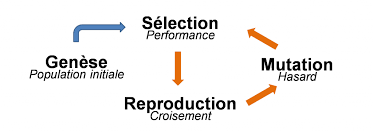
\includegraphics{.ressources/algo_gen_scheme.png}

\hypertarget{suxe9lection}{%
\subsubsection{Sélection}\label{suxe9lection}}

L'algorithme sélectionne un certain nombre d'individu (ou part de la
population définie) arbitrairement. Les individus sélectionnés subiront
les phases suivantes de croisement et mutation. La façon dont les
individus sont sélectionnés peut varier :

\begin{enumerate}
\def\labelenumi{\arabic{enumi}.}
\tightlist
\item
  \textbf{Aléatoire simple} : On sélectionne les individus de manière
  totalement aléatoire. Elle peut permet d'obtenir une sélection
  difforme et variée et d'ainsi varier les individus qui suivront.
\item
  \textbf{Aléatoire pondéré} : On attribue à chaque individu une
  \texttt{valeur\ sélective} puis, en se basant sur celle-ci,
  sélectionne les individus de manière aléatoire. Aussi, un individu
  dont la valeur est plus élevée aura plus de chance d'être sélectionné.
  \emph{Il est important de garder en tête que l'algorithme ne doit pas
  être "sur-sélectif". Il n'est donc pas pertinent de rendre la valeur
  des individus les moins évalués nulle afin de leur donner une chance
  d'être sélectionné, évoluer et éventuellement s'améliorer.} Elle
  permet d'obtenir une sélection difforme et variée tout en privilégiant
  les gènes les plus efficients sans ignorer les moins efficients.
\item
  \textbf{Prédéterminée} : On attribue un nombre (ou pourcentage)
  déterminé lors du lancement de l'algorithme qui sélectionnera (en
  fonction de ce nombre ou pourcentage) les individus parmi une part
  préalablement déterminée de la population (en fonction de leur
  évaluation). \emph{Entre autre, il sera opportun d'effectuer notre
  sélection en grand majorité parmi la population la mieux évalués, et
  parmi la population dont l'évaluation est moyenne et faible.}
\end{enumerate}

\begin{quote}
\textbf{Note :} La méthode prédéterministe peut être mixée avec les
méthodes aléatoires. La méthode de sélection peut différer en fonction
du résultat escompté. On privilégiera dans ce projet la méthode de
\textbf{sélection aléatoire pondérée}.
\end{quote}

\hypertarget{croisement}{%
\subsubsection{Croisement}\label{croisement}}

Parmi la population sélectionnée par la phase précédente, l'algorithme
effectue un croisement de gène. Celui-ci peut se faire entre deux
individus ou plus (principalement 2). Cette phase permet de produire une
population (dont les individus sont principalement bien évaluée) dont
les gènes sont croisés et diversifié par rapport à la population de
départ. \emph{La persistence des individus dont les performances sont
faibles ou moyennes leur permet de s'améliorer grâce aux individus les
mieux évalués.}

\begin{quote}
\textbf{Note :} Usuellement, la population d'entrée \texttt{a} est
supprimée et remplacée par la population de sortie \texttt{b}. Il faut
donc que cette phase produise pour des croisements entre \texttt{n}
individus, \texttt{n} individus croisés afin de garder une population au
même nombre que celle d'entrée.
\end{quote}

\begin{quote}
\textbf{Vocabulaire :}

\begin{itemize}
\tightlist
\item
  \emph{Elément d'un gène :} Prenant un gène de type chaîne de
  caractères, un caractère est un élément du gène.
\item
  \emph{Partie d'un gène :} Une partie d'un gène est une section
  découpée du gène de \texttt{x} élément.
\end{itemize}
\end{quote}

Les méthodes de croisement d'individus existent sous plusieurs formes :

\begin{enumerate}
\def\labelenumi{\arabic{enumi}.}
\tightlist
\item
  \textbf{Aléatoire simple} : Chaque élément (ou partie) du gène des
  \texttt{n} individus sont parcourus afin de produire un individu.
  L'algorithme choisi aléatoirement l'élément (ou partie) de l'individu
  \texttt{A}, \texttt{B}, etc. Cela produit alors un nouveau gène mêlant
  les éléments (ou parties) de l'individu \texttt{A}, \texttt{B}, etc.
  Cette opération est effectuée \texttt{n} fois afin de produire une
  population de quantité équivalente.
\item
  \textbf{Aléatoire hiérarchisé (ou pondéré)} : On considère que chaque
  type de gène dispose d'une coefficient (ou \texttt{valeur\ sélective}
  à la manière d'un individu). Ce dernier est utilisé comme base afin de
  pondérer le choix entre les gènes des individus croisés. Un gène à
  coefficient élevé a des chances plus élevées d'être sélectionné. Il en
  existe deux formes :

  \begin{itemize}
  \tightlist
  \item
    \textbf{Statique} : Ici, les gènes disposent d'une hiérarchie (dont
    les valeurs sont fixées arbitrairement au départ de la simulation).
    Chaque élément du gène des individus possèdent un coefficient qui
    identifie son niveau par rapport à un autre. Par exemple, la
    hiérarchie \texttt{G\textgreater{}B\textgreater{}N} (dont les
    coefficients sont \texttt{3\textgreater{}2\textgreater{}1}) où
    \texttt{B=2} est supérieur à \texttt{N=1} mais inférieur à
    \texttt{G=3}. De la même manière qu'une méthode de sélection
    aléatoire pondérée, l'algorithme choisi un élément aléatoirement
    entre l'individu \texttt{A} et \texttt{B} où l'élément dont la
    valeur hiérarchique est supérieure a plus de chance d'être
    sélectionnée.
  \item
    \textbf{Dynamique} : Cette méthode reprend le fonctionnement de la
    méthode de croisement aléatoire pondéré statique mais dans laquelle
    la hiérarchie des gènes n'est pas statique mais dynamique.
    C'est-à-dire qu'elle évolue à chaque génération et chaque population
    en fonction des gènes de cette dernière. Ainsi, une population dans
    laquelle le gène \texttt{G} est dominant verra sa hiérarchie telle
    que \texttt{G\textgreater{}...} Bien entendu, il est possible
    d'effectuer un \emph{décalage} entre une génération \texttt{n} et
    une génération \texttt{n+k} tel que : \texttt{h(n)} de \texttt{p(n)}
    est utilisée sur \texttt{p(n+1)} où \texttt{h} (hiérarchie),
    \texttt{p} (population), \texttt{n} (numéro de génération) et
    \texttt{k} (nombre de génération de décalage). Le dynamisme d'une
    hiérarchie peut se décliner sous deux formes :

    \begin{itemize}
    \tightlist
    \item
      \textbf{Dynamisme général} : Une population possède une hiérarchie
      commune. Celle-ci est recalculée au début de la phase de
      croisement en fonction de la quantité du gène au sein de la
      population totale ou sélectionnée.
    \item
      \textbf{Dynamisme unitaire} : Pour une population avec un gène de
      \texttt{k} élément, il existe \texttt{k} hiérarchie recalculée au
      début de la phase de croisement pour chaque \texttt{k}ème élément
      \texttt{e} du gène \texttt{G} (noté \texttt{e{[}k{]}}) qui dispose
      d'une hiérarchie de l'élément \texttt{k} notée
      \texttt{h(e{[}k{]})} dont le dynamisme évolue en fonction de la
      quantité des gènes de la popoulation du \texttt{k}ème élémént.
      \emph{Soit la hiérarchie \texttt{h(e{[}1{]})}, la hiérarchie de
      l'élément \texttt{1}.}
    \end{itemize}
  \end{itemize}
\end{enumerate}

\hypertarget{mutation}) en un autre gène
déterminé aléatoirement. Cette phase a pour but de donner une chance
d'évolution et de diversification à la population.

\hypertarget{objectif}{%
\subsection{Objectif}\label{objectif}}

L'objectif du principe de sélection naturelle est donc de déterminer
l'individu le plus efficient et efficace et obtenir une solution rapide
à une situation.

\begin{quote}
\textbf{Note :} Il est possible de coupler cet algorithme à un réseau de
neurones artificiels ou
\href{https://fr.wikipedia.org/wiki/R\%C3\%A9seau_de_neurones_artificiels}{\emph{Neural
Network}} basé sur les idées du psychologue
\href{https://fr.wikipedia.org/wiki/Frank_Rosenblatt}{\emph{Franck
Rosenblatt}}. Notamment pour le calcul des poids de neurones.
\emph{Quelques lectures peuvent être trouvées à ce sujet dont (en
anglais) :}

\begin{itemize}
\tightlist
\item
  \href{https://arxiv.org/pdf/1606.04393.pdf}{\emph{"Deep Learning with
  Darwin: Evolutionary Synthesis of Deep Neural Networks"}} de M. J.
  Shafiee, A. Mishra et A. Wong;
\item
  \href{https://link.springer.com/chapter/10.1007/1-4020-8151-0_6}{\emph{"Evolutionary
  Robot Behaviors Based on Natural Selection and Neural Network"}} dans
  \emph{Artificial Intelligence Applications and Innovations} de M.
  Bramer et V. Devedzic;
\item
  \href{https://home.fnal.gov/~souvik/Brain/index.html}{\emph{"Evolving
  Neural Networks"}} et
  \href{https://home.fnal.gov/~souvik/Brain/BrainInWorld.pdf}{\emph{"A
  biology-inspired neural network evolving through natural selection"}}
  de Souvik Das ;
\end{itemize}

Ou encore, un jeu de simulation
\href{https://leocaussan.itch.io/the-bibites}{\emph{"The Bibites"}}
développé par Léo Caussan dont le développement peut être suivi depuis
sa chaîne
\href{https://www.youtube.com/channel/UCjJEUMnBFHOP2zpBc7vCnsA}{YouTube}.
\end{quote}

L'objectif de ce projet est :

\begin{itemize}
\tightlist
\item
  D'une première part, \textbf{produire} un algorithme et une structure
  algorithmique permettant de calculer et \textbf{simuler} l'évolution
  d'une population d'individus dans un environnement pré-déterminé;
\item
  D'une seconde part, \textbf{observer} leur comportement afin d'en
  extrapoler des résultats que nous tenterons d'expliquer et d'évaluer.
\end{itemize}

Dans un environnement déterminé surnommé \texttt{problème}, des
individus surnommés \texttt{solutions} sont confrontés afin de
déterminer lequel, selon des critères donnés, a le plus de valeur et
sera sélectionné pour l'environnement confronté à le surmonter.

\textbf{En d'autres mots,} pour un problème établi, nous émettons des
"\emph{hypothèses}" de solutions qui, au fur et à mesure de la
simulation, établieront selon leur évaluation leur efficacité à résoudre
le problème édicté. \emph{On peut considérer que la solution de chaque
individu est un gène \texttt{G} qui leur est inné et qu'ils peuvent
transmettre, croiser et muter}.

Cette situation, bien que relativement simple, peut avoir des
applications variées. Qu'il s'agisse d'une simulation naturelle ou d'un
environnement économique où les individus sont des entreprises.

Il est important de garder en tête que l'algorithme et toutes les phases
qui le composent, notamment les phases de sélection, mutation et
croisement, doivent être optimisés. Etant donné qu'un algorithme
génétique se base sur une population avec un nombre élevé pour avoir un
résultat adéquat.

\hypertarget{duxe9roulement}{%
\section{Déroulement}\label{duxe9roulement}}

\hypertarget{cas-concret}{%
\subsection{Cas concret}\label{cas-concret}}

Afin d'obtenir les résultats escomptés par l'objectif de ce projet, il
est opportun de réaliser un exercice. Avant de produire un algorithme
génétique généralisant les cas d'utilisation d'une évolution, nous
pouvons nous consacrer à la réalisation d'un cas concret et spécifique
afin de l'utiliser comme base du cas général. Comme cas concret, nous
prendrons le suivant :

\textbf{Environnement} : Nous disposons d'un plateau de \texttt{W\ x\ W}
cases. Chaque case peut contenir \texttt{Pièce} ou pas (\emph{Ces pièces
sont au nombre \texttt{nbPiece} réparties aléatoirement sur le
plateau}). D'une position initiale \texttt{X} du pion \texttt{Pion} et
d'un entier \texttt{n}.

\textbf{Problème} : \emph{Quel est l'enchaînement de mouvement/pas
\texttt{M} à partir de la position \texttt{X} qui permet de récupérer le
plus de \texttt{Pièce} avec \texttt{n} pas ?}

\textbf{Mouvement} : Un mouvement \texttt{M} peut être \textbf{H}aut,
\textbf{B}as, \textbf{G}auche, \textbf{D}roite relatif à la position
actuelle de \texttt{Pion} et à l'axe du plateau. Un mouvement \texttt{M}
est valide tant qu'il ne fait pas sortir le pion en dehors des limites
du plateau.

\textbf{Individu} : Chaque \emph{individu} de la population contiendra
une solution/gène \texttt{G} : une suite de \texttt{n} caractère(s)
chacun représentant un mouvement/pas de type \texttt{M}.

\textbf{Evaluation} : Chacun \emph{individu} sera évalué et obtiendra un
capital d'évaluation ou \texttt{valeur\ sélective} qui sera calculée en
fonction du nombre de \texttt{Pièce} qu'il aura effectué, de la distance
parcourue entre chacune et, éventuellement, du nombre de mouvement
invalide. \emph{Il sera opportun d'évaluer chaque individu par rapport à
la performance d'autrui en gardant en tête que l'évaluation de l'un ne
devrait pas être équivalente à un autre même s'ils ont collectés le même
nombre de pièces.}

\hypertarget{gestion-du-code}{%
\subsubsection{Gestion du code}\label{gestion-du-code}}

Qu'il s'agisse de la phase de versionning ou de travail collaboratif,
plusieurs plateformes seront utilisées afin de permettre un partage
efficace du code. En outre, nous avons utilisé, utilisons ou avons tenté
d'utiliser des applications telles que :

\begin{itemize}
\tightlist
\item
  \textbf{Github} (principalement);
\item
  \textbf{Floobits} (plateforme de codage collaboratif en temps réel);
\end{itemize}

Nous avons utilisé également un package implémenté dans Java dans notre
code ou afin de tester l'application : \emph{Junit} pour produire des
tests unitaires et vérifier le fonctionnement de nos méthodes et
fonctions.

\hypertarget{architecture-du-code}{%
\subsubsection{Architecture du code}\label{architecture-du-code}}

L'architecture du code se base sur la logique orientée objet du langage
Java qui sera utilisé pour le développement de l'algorithme génétique.
Afin de rendre la structure du code générale à toute sorte d'application
de l'algorithme, il sera opportun d'utiliser des classes
\textbf{abstraites} ou des \textbf{interfaces} (vues en cours de
\emph{Programmation orientée objet}) et l'intégration des fonctions
essentielles à l'exécution de l'algorithme.

\hypertarget{classes}{%
\subsubsection{Classes}\label{classes}}

Visiblement, nous aurons besoin d'au moins deux classes pour
l'environnement (\texttt{Plateau}) et l'individu (\texttt{Pion}). A
partir de cette situation, il nous est possible d'identifier plusieurs
classes permettant la réalisation de cet algorithme :

\begin{itemize}
\tightlist
\item
  \texttt{Plateau} ;
\item
  Et \texttt{Individu}.
\end{itemize}

Les relations des classes peuvent être exprimées avec le schéma suivant
:

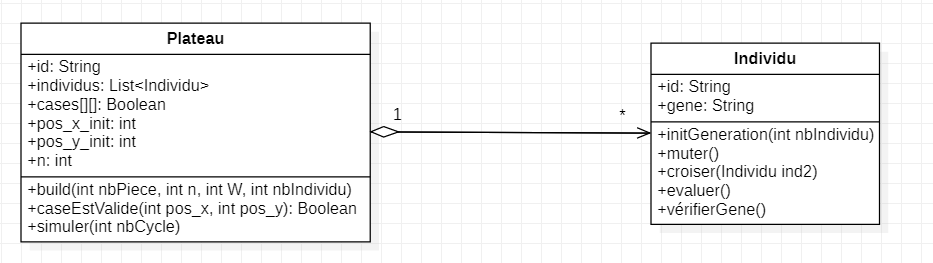
\includegraphics{.ressources/uml_classes_plateau_1.png}

Eventuellement, il est possible de créer également d'une classe
intermédiaire qui se chargent du contrôle de chaque étape de
vérification : \texttt{Mouvement}. Mais il est préférable de se tenir
aux deux classes ci-dessus pour le moment.

\end{document}
